\section{Codificando Vídeos}

Para codificar os vídeos para o \acrshort{LCEVC}, foi usando um codificador chamado
LTM Model Encoder e Decoder, obtido através do Git da MPEG. Para codificar um vídeo utilizando
este codificador, são passados os parâmetros pela linha de comando, ou
através de um arquivo de configuração que possui os valores padrões do
codificador. Como mencionado anteriormente, o \acrshort{LCEVC} é constituído por
duas camadas, a camada base contendo o um vídeo com a metade da resolução
do vídeo original, e uma camada de aprimoramento, que possui as informações
para que o \acrshort{LCEVC} possa realizar um upscaling no vídeo para que ele fique
o mais parecido com o vídeo original possível. A camada base pode estar
nos formatos AVC, VVC, HEVC e EVC. Já a camada de aprimoramento, possui
duas subcamadas, onde uma é opcional e a outra é obrigatória, contendo
os principais dados.

Para este trabalho, foi alterado o parâmetro que determina
a quantidade da qualidade que será destinada para esta subcamada. Este
valor determina a quantização desta camada, onde o quanto menor o valor,
melhor a qualidade que esta camada possuirá, consequentemente aumentando
o tamanho que a camada do \acrshort{LCEVC} terá em relação ao arquivo final. Este
valor é chamado de \textit{SW2}, e seu parâmetro é 
\texttt{-{}-cq\_step\_width\_loq\_0}. Além do valor de \textit{SW2} que
modifica a qualidade da camada do \acrshort{LCEVC}, foi modificado o valor do \textit{QP}
para a camada base. Para cada valor de \textit{QP}, foi usado uma sequência 
de valores fixos para o \textit{SW2}, para que fosse possível comparar a
relação que estes valores iriam influenciar na qualidade e tamanho final
do arquivo.
 
\section{Testes}

Neste trabalho, será analisado o resultado de várias codificações utilizando o
\acrshort{LCEVC}, para tentar demonstrar qual seriam os melhores parâmetros para o seu uso,
levando em consideração os seus casos de uso. O programa utilizado foi compilado
para Linux e sempre utilizado em uma distribuição Linux com base em Ubuntu.

Foi desenvolvido um \textit{script} \textit{Bash} para Linux que executa o programa codificador
paralelamente para cada valor de \textit{QP} utilizado. O \textit{script} cria uma execução por
\textit{QP} e processa sequencialmente por valor de \textit{SW2}. Os valores utilizados
foram:

\begin{description}
\item[QPs:] 22, 25, 27, 30, 32, 35, 37.
\item[SW2:] 250, 750, 1250, 1750, 2250, 2750, 3250.
\end{description}

Além das codificações utilizando \acrshort{LCEVC}, também foram codificados vídeos no mesmo
padrão de compressão utilizado pelo \acrshort{LCEVC}, mas sem o \acrshort{LCEVC}, para que fosse possível 
ter uma referência da qualidade máxima possível obter sem o \acrshort{LCEVC}. Neste caso, foram usados
os mesmos valores de \textit{QP} e utilizado a resolução final que o vídeo do \acrshort{LCEVC} teria.
Também foram extraídos os parâmetros que o LCEVC altera para o \textit{downsampling} da camada
base e adicionados no comando de execução da codificação sem o \acrshort{LCEVC}.
 
Por fim, também é realizado uma codificação usando somente o algoritmo base de \textit{Downsampling}
e \textit{Upsampling} que o codificador \acrshort{LCEVC} utiliza. Porém, não há interferência de nenhum padrão
de compressão neste estágio, onde ele transforma um YUV, um formato bruto de vídeo, em outro YUV. Por isso
seu \textit{bitrate} não é considerado.

Após cada vídeo ser codificado, o \textit{script} também faz o cálculo de \acrfull{PSNR} do resultado obtido,
transformado em YUV, arquivo original bruto, que também está em YUV.

\section{Fronteira de Pareto}

A \textit{Fronteira de Pareto} é uma técnica utilizada para analisar a relação entre dois ou mais
objetivos, onde é possível identificar quais soluções são eficientes em relação a
outros objetivos \cite{pareto_definition}. Neste trabalho, a Fronteira de Pareto é utilizada para analisar a relação
entre a qualidade do vídeo, medida pelo \acrshort{PSNR}, e o tamanho do arquivo, medido pelo \textit{bitrate}.
A Fronteira de Pareto é representada por um conjunto de pontos que não podem ser melhorados em um
objetivo sem piorar outro objetivo. Ou seja, se um ponto está na fronteira de Pareto, não é possível
aumentar a qualidade do vídeo sem aumentar o tamanho do arquivo, ou diminuir o tamanho do arquivo sem
diminuir a qualidade do vídeo.

\begin{figure}[h]
    \centering
    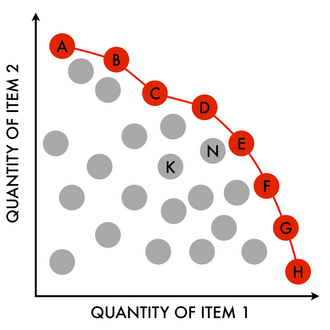
\includegraphics[width=0.5\textwidth]{img/pareto-2.png}
    \caption{Exemplo da Fronteira de Pareto. \cite{pareto_img}}
    \label{fig:pareto}
\end{figure}